\section{System Disk Encryption}
An encrypted system disk prevents that the data contained in it can be cloned or replicated without the passphrase or authentication server. For this design, the disks will be encrypted through a kickstart passphrase and then removed once the remote Tang server is reached. If a non-authorized user gains physical access to the server:
\begin{itemize}
  \item If halted and attempted to change the root password, the encryption passphrase prompt will be requested - which was deleted.
  \item If booted through a Live USB OS, the encrypted partitions remain unreadable.
  \item If the drive is removed/stolen, the disk's data remains cyphered.
\end{itemize}

\newpage
\subsection{LUKS - Linux Unified Key Setup}

According to a paper subscribed by Danut Anton and Emil Simion \footnote[1]{https://ieeexplore-ieee-org.usm.idm.oclc.org/stamp/stamp.jsp?tp=\&arnumber=8678978}, LUKS is one of the most common FDE solutions for Linux-based systems.
FDE works by encrypting every single bit on a storage device, so if the user doesn't have the password, data cannot be recovered. The most common problem for FDE solutions is password management, which at what concerns this implementation, will be handled by a two-level key hierarchy. A strong master key is generated by an OS, which is used to encrypt/decrypt the hard drive. That key has to be split and encrypted with a secret user key and stored on the device, at the beginning of the memory. The advantage of this approach is that you can have multiple systems with multiple keys, allowing you to have multiple decryption Servers.

\vskip 2cm
\begin{figure}
  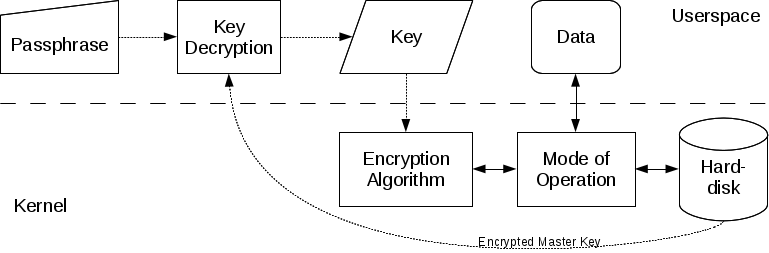
\includegraphics[width=14cm]{images/image2.png}
  \centering
  \caption{LUKS Operational Diagram}
\end{figure}

\newpage
\subsection{Clevis}

Clevis is a pluggable framework for automated decryption. It can be used to provide automate decryption of data or even automated unlocking of LUKS volumes \footnote[2]{https://github.com/latchset/clevis}.
Once Clevis has subscribed the decryption to a server, the encryption passphrase is removed, which means in a lost communication event, the server won't be able to decrypt, not even with the passphrase. To prevent this Clevis can subscribe up to 8 keys to 8 different servers/users and it can be restricted to how many of them are required as a minimum. If you set a value t=2, means that at least 2 servers have to be available at the moment of decryption.


\subsection{Clevis Puppet Profile}
\begin{lstlisting}[language=Java]
#Clevis Profile
class profile::core::clevis() {
  $packages = [
    'clevis',
    'clevis-luks',
    'clevis-dracut'
  ]

  ##Add require packages
  package { $packages:
    ensure => 'present',
  }
  ->exec { '/sbin/dracut -f --regenerate-all':
    path   => ['/usr/bin', '/sbin'],
    onlyif => 'test ! -f /usr/lib/dracut/modules.d/60clevis/clevis-hook.sh'
  }
}
\end{lstlisting}

This profile installs the clevis packages needed to encrypt and manage the LUKS encryption drives. This is not quite required, because the clevis packages are being installed during provisioning, but, it grants some useful tools like 'cryptosetup' to check the subscribed Tang servers.

\newpage
\section{Tang Server - Decryption Server}

\subsection{Tang Service}

Tang \footnote[3]{https://github.com/latchset/tang} is a server for binding data to network presence. In simple terms: you have some data, but you only want it to be available when the system containing the data is on a certain, usually secure, network, This is where Tang comes in.
First, the client gets a list of the Tang server's advertised asymmetric keys. This can happen online by a simple HTTP GET.
Second, the client uses one of these public keys to generate a unique, cryptographically strong encryption key. The data is then encrypted using this key. Once the data is encrypted, the key is discarded. Some small metadata is produced as part of this operation which the client should store in a convenient location. This process of encrypting data is the provisioning step.
Third, when the client is ready to access its data, it simply loads the metadata produced in the provisioning step and performs an HTTP POST to recover the encryption key. This process of encrypting data is the provisioning step.

\vskip 2cm
\begin{figure}
  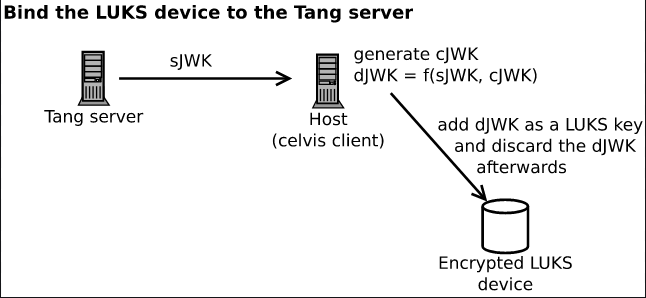
\includegraphics[width=14cm]{images/image3.png}
  \centering
  \caption{LUKS device interaction with Tang Server}
\end{figure}

\newpage
\subsection{Tang Puppet Profile and Role}

\begin{lstlisting}[language=Java]
# Tang Server Encryption Module

class profile::core::tang() {
  #Variables
  $packages = [
    'tang'
  ]

  #Add require packages
  package { $packages:
    ensure => 'present',
  }

  systemd::dropin_file {'override.conf':
    unit    => 'tangd.socket',
    content => @(OVERRIDE/L)
      [Socket]
      ListenStream=7500
      | OVERRIDE
  }
  # Ensure tang service is running
  ->service { 'tangd.socket':
    ensure  => 'running',
    require => Package[$packages],
  }
}
\end{lstlisting}

Tang profile handles the installation of the tangd.socket service, and then modifies it so it listens on port 7500 for incoming connections from clevis-dracut.

\newpage
\section{Lab Testing - Proof of Concept}
\subsection{Kickstart Modifications - Use of Encryption in Provisioning Template}
Since the drive must be encrypted with LUKS early during the provisioning, new Kickstart Provisioning Template and Partition Tables had to be created at Foreman.

\vspace*{0.1mm}
\begin{lstlisting}[language=bash]
#  Encrypted VDA - Partition Table
ignoredisk --only-use=${BOOT_DEV}
zerombr
clearpart --drives=${BOOT_DEV} --all --initlabel
part /boot     --size=1024 --asprimary --ondrive=${BOOT_DEV}
part /boot/efi --size=200  --asprimary --ondrive=${BOOT_DEV} --fstype=efi
#  Use an easy passphrase, it will be removed one step later
part pv.boot   --size=1 --grow  --encrypted --passphrase=******** --ondisk=${BOOT_DEV}
volgroup ${BOOT_VG} pv.boot
logvol /               --vgname=${BOOT_VG} --size=1 --grow --name=root
\end{lstlisting}
\vspace*{0.1mm}
"Encrypted VDA" initialize the System disk with two regular partitions - /boot and /boot/efi - and then a PV, a VG and a LV, been the LV encrypted through LUKS with a temporary password
\vspace*{0.1mm}
\begin{lstlisting}
##Kickstart - Encrypted Provisioning Template
#Packages Section
%packages
clevis-dracut
#Post Section - At ******** use the same passphrase written at the Partition Table
%post --log=/mnt/sysimage/root/install.post.log
curl -sfg http://tang01.cp.lsst.org/adv -o adv1.jws
clevis luks bind -f -k- -d /dev/vda3 \
tang '{"url":"http://tang01.cp.lsst.org","adv":"adv1.jws"}' <<< "********"
curl -sf http://tang02.cp.lsst.org/adv -o adv2.jws
clevis luks bind -f -k- -d /dev/vda3 \
tang '{"url":"http://tang02.cp.lsst.org","adv":"adv2.jws"}' \ <<< "********"
cryptsetup luksRemoveKey /dev/vda3 <<< "********"
\end{lstlisting}
\vspace*{0.1mm}
In the packages section, clevis-dracut is installed, to then be used at post to communicate with a Tang server(s), subscribe to them and remove the temporary password.

\newpage
\subsection{Test Environment}
\begin{itemize}
  \item Two Tang servers using the tang puppet profile.
  \item A client with the clevis puppet profile.
  \item The client VM (clevis01.cp.lsst.org) is provisioned through PXE with 'Encrypted VDA' Partitioning Table and 'Kickstart Encrypted Provisioning Template'.
  \item During partition creation, clevis01 root partition is encrypted through LUKS with a passphrase.
  \item Then at packages, clevis-dracut is installed to then communicate with the Tang servers at post section.
  \item At post, clevis01 subscribes to the Tang servers (tang01.cp.lsst.org and tang02.cp.lsst.org) and the temporary passphrase encryption key is removed as a decryption mechanism.
\end{itemize}

\begin{figure}
  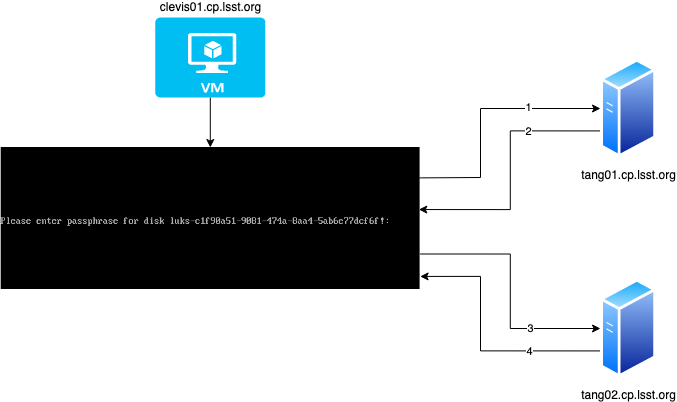
\includegraphics[width=10cm]{images/image4.png}
  \centering
  \caption{Booting procedure for an enrolled or newly enrolled client.}
\end{figure}

\begin{enumerate}
  \item During boot, the client machine attempts to reach the first Tang server.
  \item If reached, the decryption server hands over the decryption key.
  \item If the first Tang server wasn't reachable, it attempts with the next one in the key slot.
  \item The second Tang server sends the decryption key.
\end{enumerate}

\newpage
\subsection{Lab Results}
\begin{itemize}
  \item The encrypted client clevis01 successfully decrypt during dracut by reaching tang01.
  \item The primary Tang server (tang01) was powered off and the client was able to decrypt through tang02.
  \item Both Tang servers were powered off and the server remains on hold requesting a passphrase (which doesn't exist) until at least one of the Tang servers is back online (Figure 3).
  \item For the scope of this PoC, the deletion and recreation of one or both Tang servers was not done, but presumably the client decryption would not happened and the content would be irrecoverable.
  \item One way of handling the loss of all Tang servers, is to add the keys to lsst-private repo, but key rotation is suggested by the documentation to increase safety.
\end{itemize}

\begin{figure}
  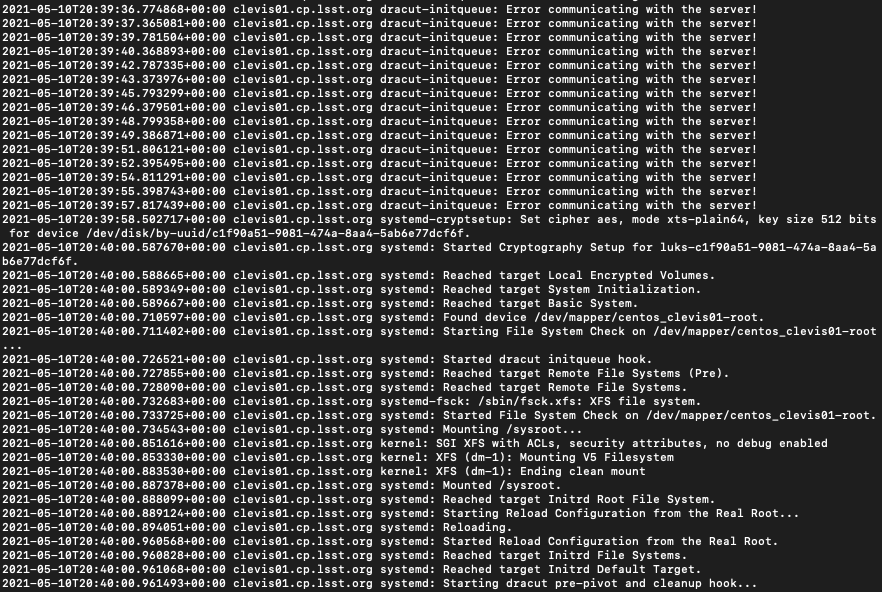
\includegraphics[width=16cm]{images/image1.png}
  \centering
  \caption{Access to LUKS encrypted drive while Tang server is rebooting}
\end{figure}

\newpage
\subsection{Performance Test - Virtual Drive over HDD}
Besides securing your data, Encryption has an impact on performance as well. Every written bit of data has to be encrypted before written on disk, which impacts both the CPU and the Disk I/O. In modern CPU architectures, the impact is not as much as it was in the past, but disks do suffer consequences.
To test the performance impact of encryption, we are going to use \textbf{\textit{sysbench}}, an open-source tool that performs series of tests to verify systems under intensive load. To have a baseline, two CentOS VM, with the same specs, were deployed: one encrypted with LUKS and a regular not encrypted one.
\subsubsection{CPU Benchmark}
\begin{center}
  Test: \textbf{\textit{sysbench --test=cpu --cpu-max-prime=20000 run}}  
\end{center}
\vspace*{-\baselineskip}
\noindent\begin{minipage}[t]{0.45\linewidth}
  \centering
  \textit{Encrypted}
  \begin{lstlisting}[basicstyle=\tiny,frame=single, numbers=left, label=cpu_test1]
  sysbench 1.0.17 (using system LuaJIT 2.0.4)  
  Running the test with following options:
  Number of threads: 1
  Initializing random number generator
  from current time
  Prime numbers limit: 20000
  Initializing worker threads...
  Threads started!
  
  CPU speed:
    events per second:   314.14
  
  General statistics:
    total time:               10.0028s
    total number of events:   3143
  
    Latency (ms):
      min:                 3.16
      avg:                 3.18
      max:                 5.40
      95th percentile:     3.19
      sum:                 10000.49 
  Threads fairness:
    events (avg/stddev):         3143.0000/0.00
    execution time (avg/stddev): 10.0005/0.00        
  \end{lstlisting}
\end{minipage}
\hspace{0.5cm}
\noindent\begin{minipage}[t]{0.45\linewidth}
  \centering
  \textit{Not-Encrypted}
  \begin{lstlisting}[basicstyle=\tiny,frame=single, label=cpu_test2]
  sysbench 1.0.17 (using system LuaJIT 2.0.4)
  Running the test with following options:
  Number of threads: 1
  Initializing random number generator
  from current time
  Prime numbers limit: 20000
  Initializing worker threads...
  Threads started!

  CPU speed:
    events per second:   314.05

  General statistics:
    total time:              10.0025s
    total number of events:  3142

    Latency (ms):
        min:               3.16
        avg:               3.18
        max:               5.21
        95th percentile:   3.19
        sum:               9995.36
  Threads fairness:
    events (avg/stddev):         3142.0000/0.00
    execution time (avg/stddev): 9.9954/0.00
  \end{lstlisting}
\end{minipage}

The results help us know that the CPU architecture, threads, and processing are the same for both VM, which will help us determine the accuracy for the following tests.
\newpage
\subsubsection{Disk Benchmark}
\begin{center}
  Test: \textbf{\textit{time sysbench --test=fileio --file-total-size=30G --file-num=24 prepare}}  
\end{center}
\vspace*{-\baselineskip}
\noindent\begin{minipage}[t]{0.45\linewidth}
  \centering
  \textit{Encrypted}
  \begin{lstlisting}[basicstyle=\tiny,frame=single, numbers=left, label=cpu_test1]
  sysbench 1.0.17 (using system LuaJIT 2.0.4)

  24 files, 1310720Kb each, 30720Mb total
  Creating files for the test...
  Extra file open flags: (none)
  Creating file test_file.0
  Creating file test_file.1
  Creating file test_file.2
  Creating file test_file.3
  Creating file test_file.4
  Creating file test_file.5
  Creating file test_file.6
  Creating file test_file.7
  Creating file test_file.8
  Creating file test_file.9
  Creating file test_file.10
  Creating file test_file.11
  Creating file test_file.12
  Creating file test_file.13
  Creating file test_file.14
  Creating file test_file.15
  Creating file test_file.16
  Creating file test_file.17
  Creating file test_file.18
  Creating file test_file.19
  Creating file test_file.20
  Creating file test_file.21
  Creating file test_file.22
  Creating file test_file.23
  32212254720 bytes written in 244.25 seconds (125.77 MiB/sec).
  
  real	4m4.275s
  user	0m1.205s
  sys	0m46.108s
  \end{lstlisting}
\end{minipage}
\hspace{0.5cm}
\noindent\begin{minipage}[t]{0.45\linewidth}
  \centering
  \textit{Not-Encrypted}
  \begin{lstlisting}[basicstyle=\tiny,frame=single, label=cpu_test2]
  sysbench 1.0.17 (using system LuaJIT 2.0.4)

  24 files, 1310720Kb each, 30720Mb total
  Creating files for the test...
  Extra file open flags: (none)
  Creating file test_file.0
  Creating file test_file.1
  Creating file test_file.2
  Creating file test_file.3
  Creating file test_file.4
  Creating file test_file.5
  Creating file test_file.6
  Creating file test_file.7
  Creating file test_file.8
  Creating file test_file.9
  Creating file test_file.10
  Creating file test_file.11
  Creating file test_file.12
  Creating file test_file.13
  Creating file test_file.14
  Creating file test_file.15
  Creating file test_file.16
  Creating file test_file.17
  Creating file test_file.18
  Creating file test_file.19
  Creating file test_file.20
  Creating file test_file.21
  Creating file test_file.22
  Creating file test_file.23
  32212254720 bytes written in 105.24 seconds (291.91 MiB/sec).
  
  real	1m45.253s
  user	0m1.201s
  sys	0m50.978s
  \end{lstlisting}
\end{minipage}

First, there is a preparation stage, in which several files are created, so they can be then moved, synced, copied, and deleted. Based on this operations, \textbf{\textit{sysbench}} will reflect the Disk IO times.
Yet, it is important to notice that for only writing the files, the Encrypted vs Not-Encryption rates are significantly impact: while the Not-Encrypted had a rate of 291.91 [MiB/sec], the Encrypted one was only 125.77 [MiB/sec], which result in almost tripling the amount of time required to write 30 GB.

\newpage
\begin{center}
  Test: \textbf{\textit{sysbench fileio --file-total-size=30G --file-num=24 --file-test-mode=rndrw --time=1800 --file-rw-ratio=1 --threads=16 --max-requests=0 run}}  
\end{center}
\vspace*{-\baselineskip}
\noindent\begin{minipage}[t]{0.45\linewidth}
  \centering
  \textit{Encrypted}
  \begin{lstlisting}[basicstyle=\tiny,frame=single, numbers=left, label=cpu_test1]
  Number of threads: 16
  24 files, 1.25GiB each
  30GiB total file size
  Block size 16KiB
  Read/Write ratio for combined random IO test: 1.00
  Periodic FSYNC enabled, calling fsync() each 100 requests.
  Calling fsync() at the end of test, Enabled.
  Using synchronous I/O mode
  Doing random r/w test
  Initializing worker threads...
  Threads started!

  File operations:
      reads/s:                      2755.75
      writes/s:                     2755.75
      fsyncs/s:                     1322.96
  
  Throughput:
      read, MiB/s:                  43.06
      written, MiB/s:               43.06
  
  General statistics:
      total time:                   1800.0206s
      total number of events:       12301839
  Latency (ms):
            min:                     0.00
            avg:                     2.34
            max:                     429.07
            95th percentile:         8.74
            sum:                     28757517.82
  
  Threads fairness:
    events (avg/stddev):         768864.9375/3513.22
    execution time (avg/stddev): 1797.3449/0.09
  \end{lstlisting}
\end{minipage}
\hspace{0.5cm}
\noindent\begin{minipage}[t]{0.45\linewidth}
  \centering
  \textit{Not-Encrypted}
  \begin{lstlisting}[basicstyle=\tiny,frame=single, label=cpu_test2]
  Number of threads: 16
  24 files, 1.25GiB each
  30GiB total file size
  Block size 16KiB
  Read/Write ratio for combined random IO test: 1.00
  Periodic FSYNC enabled, calling fsync() each 100 requests.
  Calling fsync() at the end of test, Enabled.
  Using synchronous I/O mode
  Doing random r/w test
  Initializing worker threads...
  Threads started!

  File operations:
      reads/s:                      6842.16
      writes/s:                     6842.16
      fsyncs/s:                     3284.45
  
  Throughput:
      read, MiB/s:                  106.91
      written, MiB/s:               106.91
  
  General statistics:
      total time:                   1800.0121s
      total number of events:       30543674
  Latency (ms):
            min:                     0.00
            avg:                     0.94
            max:                     536.87
            95th percentile:         3.36
            sum:                     28764555.92
  
  Threads fairness:
    events (avg/stddev):         1908979.6250/7247.20
    execution time (avg/stddev): 1797.7847/0.04
  \end{lstlisting}
\end{minipage}


\begin{figure}
  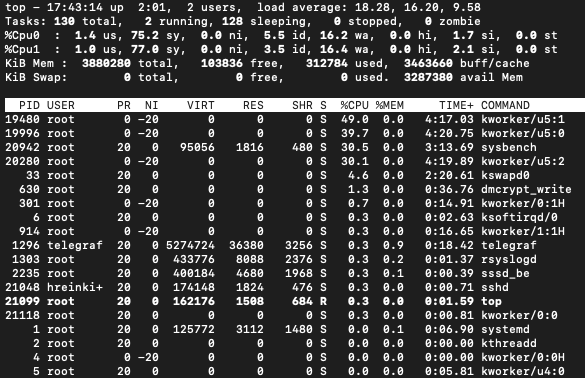
\includegraphics[width=10cm]{images/image5.png}
  \centering
  \caption{CPU Load while running sysbench}
\end{figure}

\newpage
To get a more clear view of the performance results, let's arrange them in a more comfortable way:

\begin{center}
  \tiny
  \begin{tabular}{||c c c c c||}
    \hline
    \textbf{Section} & \textbf{Metric} & \textbf{Encrypted} & \textbf{Not-Encrypted} & \textbf{Percentage} \\ [0.5ex]
    \hline
    \multirow{3}{4em}{File Operations} & reads/s & 2755.75 & 6842.16 & 40.28 \\
    & writes/s & 2755.75 & 6842.16 & 40.28 \\
    & fsyncs/s & 1322.96 & 3284.45 & 40,28 \\
    \hline
    \multirow{2}{4em}{Throughput} & reads MiB/s & 43.06 & 106.91 & 40.28 \\
    & written MiB/s & 43.06 & 106.91 & 40,28 \\
    \hline
    \multirow{2}{4em}{General Stadistics} & total time & 1800.0206[s] & 1800.0121[s] & 100.1 \\
    & total number of events & 12301839 & 30543674 & 40.28 \\
    \hline
    \multirow{5}{4em}{Latency} & min & 0 & 0 & 0 \\
    & avg & 2.34 & 0.94 & 40,17 \\
    & max & 249.07 & 536.87 & 46,4 \\
    & 95th Percentile & 8.74 & 3.36 & 38,44 \\
    & sum & 28757517.82 & 28764555.92 & 100,02 \\
    \hline
    \multirow{2}{4em}{Threads fairness} & events (avg/stddev) & 768864.9375/3513.22 & 1908979.6250/7247.20 & 40.28/48.48 \\
    & execution time (avg/stddev) & 1797.3449/0.09 & 1797.7847/0.04 & 100.02/44.44 \\
    \hline
  \end{tabular}
\end{center}

As shown in Figure 5, during the performance test at the Encrypted VM, the load on the CPU was so high (18.28) that the ssh connection was terminated and the network connection lost. As far as the results goes:
\begin{itemize}
  \item \textbf{Files Operations:} Reads, Writes, and File Sync operations suffered a ~40.3 percent due to encryption.
  \item \textbf{Throughput:} lost a ~40.3 percentage both at write and read operations while Encrypting.
  \item \textbf{General Statistics:} The number of events compared with the total time for them to occur, shows that in the same amount of time, ~40.3 percentage more events happened at the Not-Encrypted VM.
  \item \textbf{Latency:} In the same time period, the Encrypted vs Not-Encrypted suffered a ~40.17 percentage more latency.
  \item \textbf{Threads Fairness:} The number of events per thread, were ~40.28 percent higher in a Not-Encrypted system than in an Encrypted one.
\end{itemize}

\newpage
\subsection{HDD Conclusions - Pros and Cons}
\begin{itemize}
  \item Encrypting a system, results in average a 40 percent payload over the read/write operations.
  \item The encrypted client clevis01 successfully decrypt during dracut by reaching tang01.
  \item The primary Tang server (tang01) was powered off and the client was able to decrypt through tang02.
  \item For the scope of this PoC, the deletion and recreation of one or both Tang servers was not done, but presumably, the client decryption would not happen and the content would be irrecoverable.
  \item One way of handling the loss of all Tang servers is to add the keys to lsst-private repo, but key rotation is suggested by the documentation to increase safety.
\end{itemize}

\newpage
\subsection{Performance Test - Virtual Drive over GPFS/Gluster}
General Parallel File System \footnote[1]{https://es.wikipedia.org/wiki/General\_Parallel\_File\_System} is a high-performance clustered file system software developed by IBM. It provides concurrent, high-speed file access to applications executing on multiple nodes of clusters.
Gluster \footnote[2]{https://docs.gluster.org/en/latest/} is a scalable network filesystem suitable for data-intensive tasks such as cloud storage and media streaming. It is free and open-source and can utilize standard hardware. 
Since GPFS is not an open-source solution, it can not be tested for encryption performance, but GlusterFS offers the same suitable performance attributes from GPFS, and it can be easily mounted and tested. Then, for the GPFS Encryption Test, we are going to try a VM over a GlusterFS.

\subsubsection{Environment Setup - GlusterFS}
\begin{itemize}
  \item Over one ESXi hypervisor, with HDD storage, three VMs were deployed: gluster01, gluster02, and gluster03.
  \item Each VM has a 50GB storage partition and a replica three configuration, which means that meanwhile, one VM is still running, the data will be accessible. 
  \item A glusterFS pool was generated and then mounted into another ESXi hypervisor through NFS.
  \item The performance tests were performed simultaneously in both VMs (encrypted and not-encrypted) to hit as much as possible the gluster storage.
\end{itemize}
\newpage
\subsubsection{CPU Benchmark}
\begin{center}
  Test: \textbf{\textit{sysbench --test=cpu --cpu-max-prime=20000 run}}  
\end{center}
\vspace*{-\baselineskip}
\noindent\begin{minipage}[t]{0.45\linewidth}
  \centering
  \textit{Encrypted}
  \begin{lstlisting}[basicstyle=\tiny,frame=single, numbers=left, label=cpu_test1]
  Number of threads: 1
  Prime numbers limit: 20000
  Initializing worker threads...
  CPU speed:
      events per second:   350.74
  General statistics:
      total time:                          10.0028s
      total number of events:              3509
  Latency (ms):
      min:                                    2.76
      avg:                                    2.85
      max:                                    3.33
      95th percentile:                        2.97
      sum:                                10000.15
  Threads fairness:
      events (avg/stddev):           3509.0000/0.00
      execution time (avg/stddev):   10.0001/0.00
  \end{lstlisting}
\end{minipage}
\hspace{0.5cm}
\noindent\begin{minipage}[t]{0.45\linewidth}
  \centering
  \textit{Not-Encrypted}
  \begin{lstlisting}[basicstyle=\tiny,frame=single, label=cpu_test2]
  Number of threads: 1
  Prime numbers limit: 20000
  Initializing worker threads...
  CPU speed:
      events per second:   329.91
  General statistics:
      total time:                          10.0007s
      total number of events:              3300
  Latency (ms):
      min:                                    2.76
      avg:                                    3.03
      max:                                    7.87
      95th percentile:                        3.02
      sum:                                 9997.00
  Threads fairness:
      events (avg/stddev):           3300.0000/0.00
      execution time (avg/stddev):   9.9970/0.00
  \end{lstlisting}
\end{minipage}

\subsubsection{Disk Benchmark}
\begin{center}
  Test: \textbf{\textit{time sysbench --test=fileio --file-total-size=30G --file-num=24 prepare}}  
\end{center}
\vspace*{-\baselineskip}
\noindent\begin{minipage}[t]{0.45\linewidth}
  \centering
  \textit{Encrypted}
  \begin{lstlisting}[basicstyle=\tiny,frame=single, numbers=left, label=cpu_test1]
  24 files, 655360Kb each, 15360Mb total
  Creating files for the test...
  Creating file test_file.0
  Creating file test_file.1
  #
  #OMITTING OUTPUT FROM
  #FILE2 TO FILE21
  #
  Creating file test_file.22
  Creating file test_file.23
  16106127360 bytes written in 505.82 seconds (30.37 MiB/sec).
  
  real    8m25.865s
  user    0m0.385s
  sys     0m19.232s
  \end{lstlisting}
\end{minipage}
\hspace{0.5cm}
\noindent\begin{minipage}[t]{0.45\linewidth}
  \centering
  \textit{Not-Encrypted}
  \begin{lstlisting}[basicstyle=\tiny,frame=single, label=cpu_test2]
  24 files, 655360Kb each, 15360Mb total
  Creating files for the test...
  Creating file test_file.0
  Creating file test_file.1
  #
  #OMITTING OUTPUT FROM
  #FILE2 TO FILE21
  #
  Creating file test_file.22
  Creating file test_file.23
  16106127360 bytes written in 504.78 seconds (30.43 MiB/sec).
  
  real	8m25.183s
  user	0m0.360s
  sys	  0m20.746s    
  \end{lstlisting}
\end{minipage}

\newpage
\begin{center}
  Test: \textbf{\textit{sysbench fileio --file-total-size=30G --file-num=24 --file-test-mode=rndrw --time=1800 --file-rw-ratio=1 --threads=16 --max-requests=0 run}}  
\end{center}
\vspace*{-\baselineskip}
\noindent\begin{minipage}[t]{0.45\linewidth}
  \centering
  \textit{Encrypted}
  \begin{lstlisting}[basicstyle=\tiny,frame=single, numbers=left, label=cpu_test1]
  Running the test with following options:
  Number of threads: 16
  Initializing random number generator from current time
  24 files, 640MiB each
  15GiB total file size
  Block size 16KiB
  Read/Write ratio for combined random IO test: 1.00
  Periodic FSYNC enabled, calling fsync() each 100 requests.
  Calling fsync() at the end of test, Enabled.
  Using synchronous I/O mode
  Doing random r/w test
  Initializing worker threads...
  Threads started!
  File operations:
      reads/s:                      74.55
      writes/s:                     74.55
      fsyncs/s:                     36.00
  Throughput:
      read, MiB/s:                  1.16
      written, MiB/s:               1.16
  General statistics:
      total time:                          1800.1486s
      total number of events:              332823
  Latency (ms):
      min:                                    0.00
      avg:                                   86.54
      max:                                 1212.47
      95th percentile:                      363.18
      sum:                             28800880.92
  Threads fairness:
      events (avg/stddev):           20801.4375/174.99
      execution time (avg/stddev):   1800.0551/0.01
  \end{lstlisting}
\end{minipage}
\hspace{0.5cm}
\noindent\begin{minipage}[t]{0.45\linewidth}
  \centering
  \textit{Not-Encrypted}
  \begin{lstlisting}[basicstyle=\tiny,frame=single, label=cpu_test2]
  Running the test with following options:
  Number of threads: 16
  Initializing random number generator from current time
  24 files, 640MiB each
  15GiB total file size
  Block size 16KiB
  Read/Write ratio for combined random IO test: 1.00
  Periodic FSYNC enabled, calling fsync() each 100 requests.
  Calling fsync() at the end of test, Enabled.
  Using synchronous I/O mode
  Doing random r/w test
  Initializing worker threads...
  Threads started!
  File operations:
      reads/s:                      76.57
      writes/s:                     76.56
      fsyncs/s:                     36.95
  Throughput:
      read, MiB/s:                  1.20
      written, MiB/s:               1.20
  General statistics:
      total time:                          1800.4639s
      total number of events:              341849
  Latency (ms):
      min:                                    0.00
      avg:                                   84.25
      max:                                 1261.22
      95th percentile:                      363.18
      sum:                             28801639.84
  Threads fairness:
      events (avg/stddev):           21365.5625/138.94
      execution time (avg/stddev):   1800.1025/0.00
  \end{lstlisting}
\end{minipage}

\newpage
Table Comparison 
\begin{center}
  \tiny
  \begin{tabular}{||c c c c c||}
    \hline
    \textbf{Section} & \textbf{Metric} & \textbf{Encrypted} & \textbf{Not-Encrypted} & \textbf{Percentage} \\ [0.5ex]
    \hline
    \multirow{3}{4em}{File Operations} & reads/s & 74.55 & 76.57 & PERCENTAGE \\
    & writes/s & 74.55 & 76.56 & PERCENTAGE \\
    & fsyncs/s & 36.00 & 36.95 & PERCENTAGE \\
    \hline
    \multirow{2}{4em}{Throughput} & reads MiB/s & 1.16 & 1.20 & PERCENTAGE \\
    & written MiB/s & 1.16 & 1.20 & PERCENTAGE \\
    \hline
    \multirow{2}{4em}{General Stadistics} & total time & 1800.1486s & 1800.4639s & PERCENTAGE \\
    & total number of events & 332823 & 143849 & PERCENTAGE \\
    \hline
    \multirow{5}{4em}{Latency} & min & 0.00 & 0.00 & 0 \\
    & avg & 86.54 & 84.25 & PERCENTAGE \\
    & max & 1212.47 & 1261.22 & PERCENTAGE \\
    & 95th Percentile & 363.18 & 363.18 & PERCENTAGE \\
    & sum & 28800880.92 & 28801639.84 & PERCENTAGE \\
    \hline
    \multirow{2}{4em}{Threads fairness} & events (avg/stddev) & 20801.4375/174.99 & 21365.5624/138.94 & NUMBER1/NUMBER2 \\
    & execution time (avg/stddev) & 1800.0551/0.01 & 1800.1025/0.00 & NUMBER1/NUMBER2 \\
    \hline
  \end{tabular}
\end{center}

\begin{itemize}
  \item \textbf{Files Operations:} 
  \item \textbf{Throughput:} 
  \item \textbf{General Statistics:}
  \item \textbf{Latency:}
  \item \textbf{Threads Fairness:}
\end{itemize}

\subsection{GPFS Conclusions - Pros and Cons}
\begin{itemize}
  \item First
  \item Second
  \item Third...
\end{itemize}

\newpage
\subsection{Performance Test - Virtual Drive over SDD}
\subsubsection{CPU Benchmark}
\begin{center}
  Test: \textbf{\textit{sysbench --test=cpu --cpu-max-prime=20000 run}}  
\end{center}
\vspace*{-\baselineskip}
\noindent\begin{minipage}[t]{0.45\linewidth}
  \centering
  \textit{Encrypted}
  \lstset{language=bash,label=SliceExaple}
  \begin{lstlisting}[basicstyle=\tiny,frame=single, numbers=left, label=cpu_test1]
  Test Content      
  \end{lstlisting}
\end{minipage}
\hspace{0.5cm}
\noindent\begin{minipage}[t]{0.45\linewidth}
  \centering
  \textit{Not-Encrypted}
  \begin{lstlisting}[basicstyle=\tiny,frame=single, label=cpu_test2]
  Test Content
  \end{lstlisting}
\end{minipage}

\newpage
\subsubsection{Disk Benchmark}
\begin{center}
  Test: \textbf{\textit{time sysbench --test=fileio --file-total-size=30G --file-num=24 prepare}}  
\end{center}
\vspace*{-\baselineskip}
\noindent\begin{minipage}[t]{0.45\linewidth}
  \centering
  \textit{Encrypted}
  \lstset{language=bash,label=SliceExaple}
  \begin{lstlisting}[basicstyle=\tiny,frame=single, numbers=left, label=cpu_test1]
  Test Content
  \end{lstlisting}
\end{minipage}
\hspace{0.5cm}
\noindent\begin{minipage}[t]{0.45\linewidth}
  \centering
  \textit{Not-Encrypted}
  \begin{lstlisting}[basicstyle=\tiny,frame=single, label=cpu_test2]
  Test Content
  \end{lstlisting}
\end{minipage}

\newpage
\begin{center}
  Test: \textbf{\textit{sysbench fileio --file-total-size=30G --file-num=24 --file-test-mode=rndrw --time=1800 --file-rw-ratio=1 --threads=16 --max-requests=0 run}}  
\end{center}
\vspace*{-\baselineskip}
\noindent\begin{minipage}[t]{0.45\linewidth}
  \centering
  \textit{Encrypted}
  \lstset{language=bash,label=SliceExaple}
  \begin{lstlisting}[basicstyle=\tiny,frame=single, numbers=left, label=cpu_test1]
  Test Content
  \end{lstlisting}
\end{minipage}
\hspace{0.5cm}
\noindent\begin{minipage}[t]{0.45\linewidth}
  \centering
  \textit{Not-Encrypted}
  \begin{lstlisting}[basicstyle=\tiny,frame=single, label=cpu_test2]
  Test Content
  \end{lstlisting}
\end{minipage}


\begin{figure}
  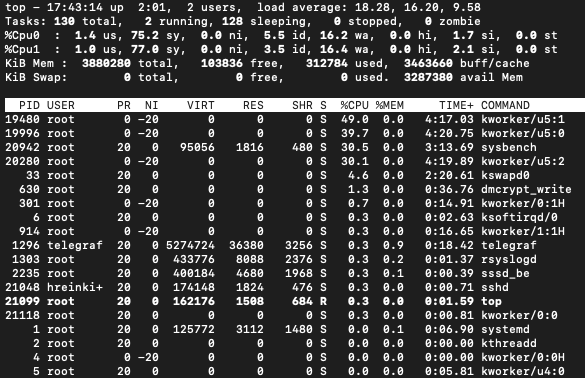
\includegraphics[width=10cm]{images/image5.png}
  \centering
  \caption{CPU Load while running sysbench}
\end{figure}

\newpage
To get a more clear view of the performance results, let's arrange them in a more comfortable way:

\begin{center}
  \tiny
  \begin{tabular}{||c c c c c||}
    \hline
    \textbf{Section} & \textbf{Metric} & \textbf{Encrypted} & \textbf{Not-Encrypted} & \textbf{Percentage} \\ [0.5ex]
    \hline
    \multirow{3}{4em}{File Operations} & reads/s & NUMBER1 & NUMBER2 & PERCENTAGE \\
    & writes/s & NUMBER1 & NUMBER & PERCENTAGE \\
    & fsyncs/s & NUMBER1 & NUMBER & PERCENTAGE \\
    \hline
    \multirow{2}{4em}{Throughput} & reads MiB/s & NUMBER1 & NUMBER2 & PERCENTAGE \\
    & written MiB/s & NUMBER1 & NUMBER2 & PERCENTAGE \\
    \hline
    \multirow{2}{4em}{General Stadistics} & total time & NUMBER1 & NUMBER2 & PERCENTAGE \\
    & total number of events & NUMBER1 & NUMBER2 & PERCENTAGE \\
    \hline
    \multirow{5}{4em}{Latency} & min & NUMBER1 & NUMBER2 & PERCENTAGE \\
    & avg & NUMBER1 & NUMBER2 & PERCENTAGE \\
    & max & NUMBER1 & NUMBER2 & PERCENTAGE \\
    & 95th Percentile & NUMBER1 & NUMBER2 & PERCENTAGE \\
    & sum & NUMBER1 & NUMBER2 & PERCENTAGE \\
    \hline
    \multirow{2}{4em}{Threads fairness} & events (avg/stddev) & NUMBER1/NUMBER2 & NUMBER1/NUMBER2 & NUMBER1/NUMBER2 \\
    & execution time (avg/stddev) & NUMBER1/NUMBER2 & NUMBER1/NUMBER2 & NUMBER1/NUMBER2 \\
    \hline
  \end{tabular}
\end{center}

Impact
\begin{itemize}
  \item \textbf{Files Operations:} 
  \item \textbf{Throughput:} 
  \item \textbf{General Statistics:}
  \item \textbf{Latency:}
  \item \textbf{Threads Fairness:}
\end{itemize}

\newpage
\subsection{SDD Conclusions - Pros and Cons}
\begin{itemize}
  \item First
  \item Second
  \item Third...
\end{itemize}

\newpage
\subsection{Performance Test - Virtual Drive over NVMe}
\subsubsection{CPU Benchmark}
\begin{center}
  Test: \textbf{\textit{sysbench --test=cpu --cpu-max-prime=20000 run}}  
\end{center}
\vspace*{-\baselineskip}
\noindent\begin{minipage}[t]{0.45\linewidth}
  \centering
  \textit{Encrypted}
  \lstset{language=bash,label=SliceExaple}
  \begin{lstlisting}[basicstyle=\tiny,frame=single, numbers=left, label=cpu_test1]
  Test Content      
  \end{lstlisting}
\end{minipage}
\hspace{0.5cm}
\noindent\begin{minipage}[t]{0.45\linewidth}
  \centering
  \textit{Not-Encrypted}
  \begin{lstlisting}[basicstyle=\tiny,frame=single, label=cpu_test2]
  Test Content
  \end{lstlisting}
\end{minipage}

\newpage
\subsubsection{Disk Benchmark}
\begin{center}
  Test: \textbf{\textit{time sysbench --test=fileio --file-total-size=30G --file-num=24 prepare}}  
\end{center}
\vspace*{-\baselineskip}
\noindent\begin{minipage}[t]{0.45\linewidth}
  \centering
  \textit{Encrypted}
  \lstset{language=bash,label=SliceExaple}
  \begin{lstlisting}[basicstyle=\tiny,frame=single, numbers=left, label=cpu_test1]
  Test Content
  \end{lstlisting}
\end{minipage}
\hspace{0.5cm}
\noindent\begin{minipage}[t]{0.45\linewidth}
  \centering
  \textit{Not-Encrypted}
  \begin{lstlisting}[basicstyle=\tiny,frame=single, label=cpu_test2]
  Test Content
  \end{lstlisting}
\end{minipage}

\newpage
\begin{center}
  Test: \textbf{\textit{sysbench fileio --file-total-size=30G --file-num=24 --file-test-mode=rndrw --time=1800 --file-rw-ratio=1 --threads=16 --max-requests=0 run}}  
\end{center}
\vspace*{-\baselineskip}
\noindent\begin{minipage}[t]{0.45\linewidth}
  \centering
  \textit{Encrypted}
  \lstset{language=bash,label=SliceExaple}
  \begin{lstlisting}[basicstyle=\tiny,frame=single, numbers=left, label=cpu_test1]
  Test Content
  \end{lstlisting}
\end{minipage}
\hspace{0.5cm}
\noindent\begin{minipage}[t]{0.45\linewidth}
  \centering
  \textit{Not-Encrypted}
  \begin{lstlisting}[basicstyle=\tiny,frame=single, label=cpu_test2]
  Test Content
  \end{lstlisting}
\end{minipage}


\begin{figure}
  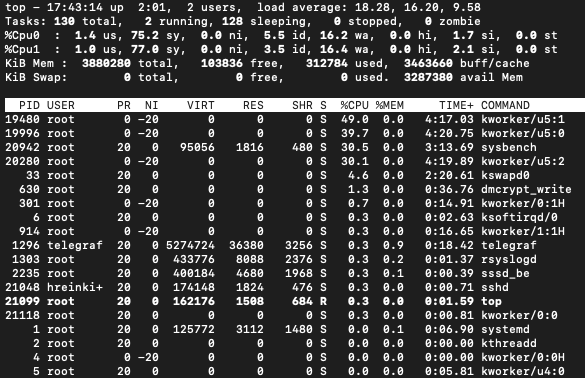
\includegraphics[width=10cm]{images/image5.png}
  \centering
  \caption{CPU Load while running sysbench}
\end{figure}

\newpage
To get a more clear view of the performance results, let's arrange them in a more comfortable way:

\begin{center}
  \tiny
  \begin{tabular}{||c c c c c||}
    \hline
    \textbf{Section} & \textbf{Metric} & \textbf{Encrypted} & \textbf{Not-Encrypted} & \textbf{Percentage} \\ [0.5ex]
    \hline
    \multirow{3}{4em}{File Operations} & reads/s & NUMBER1 & NUMBER2 & PERCENTAGE \\
    & writes/s & NUMBER1 & NUMBER & PERCENTAGE \\
    & fsyncs/s & NUMBER1 & NUMBER & PERCENTAGE \\
    \hline
    \multirow{2}{4em}{Throughput} & reads MiB/s & NUMBER1 & NUMBER2 & PERCENTAGE \\
    & written MiB/s & NUMBER1 & NUMBER2 & PERCENTAGE \\
    \hline
    \multirow{2}{4em}{General Stadistics} & total time & NUMBER1 & NUMBER2 & PERCENTAGE \\
    & total number of events & NUMBER1 & NUMBER2 & PERCENTAGE \\
    \hline
    \multirow{5}{4em}{Latency} & min & NUMBER1 & NUMBER2 & PERCENTAGE \\
    & avg & NUMBER1 & NUMBER2 & PERCENTAGE \\
    & max & NUMBER1 & NUMBER2 & PERCENTAGE \\
    & 95th Percentile & NUMBER1 & NUMBER2 & PERCENTAGE \\
    & sum & NUMBER1 & NUMBER2 & PERCENTAGE \\
    \hline
    \multirow{2}{4em}{Threads fairness} & events (avg/stddev) & NUMBER1/NUMBER2 & NUMBER1/NUMBER2 & NUMBER1/NUMBER2 \\
    & execution time (avg/stddev) & NUMBER1/NUMBER2 & NUMBER1/NUMBER2 & NUMBER1/NUMBER2 \\
    \hline
  \end{tabular}
\end{center}

Impact
\begin{itemize}
  \item \textbf{Files Operations:} 
  \item \textbf{Throughput:} 
  \item \textbf{General Statistics:}
  \item \textbf{Latency:}
  \item \textbf{Threads Fairness:}
\end{itemize}

\newpage
\subsection{NVMe Conclusions - Pros and Cons}
\begin{itemize}
  \item First
  \item Second
  \item Third...
\end{itemize}
